\scanpage{160}
% archive foliation: 159
Groupe fondamental dans les catégories.

$\mathcal C$ une catégorie, avec une famille $(D)$ de morphismes dans $\mathcal C$, satisfaisant aux conditions usuelles

(i) Contient identité et stable par composition

(ii) Stable par changement de base

On suppose de plus

(iii) \inserted{$(D)$} \unsure{Ce} sont des morphismes de descente [donc des épimorphismes stricts \inserted{universels} si \inserted{\uline{on suppose que}} \uline{les produits et produits fibrés existent}].
Enfin, on suppose

\figure{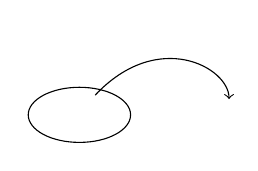
\begin{tikzpicture}[x=1cm,y=1cm]
\draw (0,0) ellipse (.65 and .35);
\draw[->] (.2,.25) .. controls (1,1.1) and (1.9,.6) .. (1.9,.2);
\end{tikzpicture}}

\margin{On peut avoir $\mathcal C$ \unsure{restreint}, en introduisant de \unsure{façon} \deleted{\unsure{connue}} une classe de morphismes $(D)$ [des morphismes \unsure{permettant} \unsure{(i), (ii)}].}

(iv) On peut ``descendre'' un $g\in(D)$ par un $f\in(D)$
[mais on ne suppose pas qu'on peut descendre \uline{tout} morphisme par un $f\in(D)$].

\uline{Dans la suite, $D$ est supposé donné une fois pour toutes.}

\uline{On suppose que dans $\mathcal C$ les sommes finies} [resp. quelconques] existent
\inserted{et \unsure{satisfont à certaines conditions}}.

\margin{\fbox{\parbox{.3\linewidth}{(v) La projection $X\times I\longrightarrow X$ est $\in(D)$.}}}

\uline{Exemple}
Catégor. $\mathcal C$ des préschémas. \deleted{La catégorie}
Classe $(D)$ des morphismes \uline{plats} et \uline{affines}.
[ou \uline{plats} et quasi-projectifs].

On va développer une théorie particulière de fibrés principaux [vérifiant les conditions générales \deleted{\unsure{correspondantes}} d'une théorie de fibrés principaux, cf. ---].

\uline{Groupes structuraux}: $X\times G$\qquad $G$ un groupe ordinaire fini [\unsure{resp.!} quelconque]

\uline{Fibrés principaux \unsure{bons} sur $X$}, de groupe $G$: les fibrés \uline{formels} ainsi, avec hom $P\to X$ $\in(D)$
